% Option C: what a linear readout can express, raw scalar vs Fourier encoding.
%   pdflatex linear_readout.tex
\documentclass[tikz,border=4pt]{standalone}
\usepackage{amsmath}
\usetikzlibrary{positioning,calc}

\begin{document}
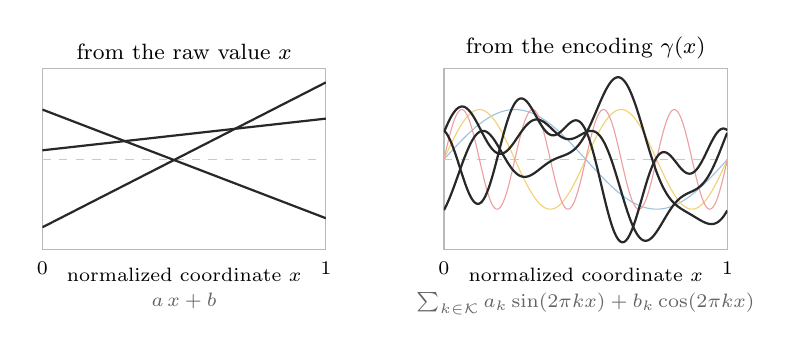
\begin{tikzpicture}[font=\small]

\definecolor{k1color}{RGB}{31,119,180}
\definecolor{k2color}{RGB}{230,171,2}
\definecolor{k4color}{RGB}{214,39,40}
\definecolor{rule}{RGB}{100,100,100}
\definecolor{curvecol}{RGB}{40,40,40}

\def\pw{3.6}   % panel width  (cm)
\def\ph{1.15}  % panel half-height (cm)
\def\gap{1.5}  % gap between panels

% ---------------- helper: axes box ----------------
\newcommand{\panelaxes}[1]{%
  \draw[rule!45, thin] (0,-\ph) rectangle (\pw,\ph);
  \draw[rule!35, thin, dashed] (0,0) -- (\pw,0);
  \node[font=\scriptsize, below=1pt] at (0,-\ph) {0};
  \node[font=\scriptsize, below=1pt] at (\pw,-\ph) {1};
  \node[font=\scriptsize, below=3pt] at (\pw/2,-\ph) {#1};
}

% =========== LEFT: raw scalar ===========
\begin{scope}
  \panelaxes{normalized coordinate $x$}
  \begin{scope}
    \clip (0,-\ph) rectangle (\pw,\ph);
    \draw[curvecol, thick]      (0,{-0.75*\ph}) -- (\pw,{0.85*\ph});
    \draw[curvecol, thick]      (0,{0.55*\ph})  -- (\pw,{-0.65*\ph});
    \draw[curvecol, thick]      (0,{0.10*\ph})  -- (\pw,{0.45*\ph});
  \end{scope}
  \node[anchor=south, font=\footnotesize] at (\pw/2,\ph) {from the raw value $x$};
  \node[anchor=north, font=\scriptsize, text=rule] at (\pw/2,{-\ph-0.42}) {$a\,x + b$};
\end{scope}

% =========== RIGHT: Fourier encoding ===========
\begin{scope}[xshift={(\pw+\gap)*1cm}]
  \panelaxes{normalized coordinate $x$}
  \begin{scope}
    \clip (0,-\ph) rectangle (\pw,\ph);
    % faint individual harmonics, coloured as in Fig. 2
    \draw[k1color!45, thin] plot[domain=0:1, samples=200, variable=\x]
      ({\x*\pw},{0.55*\ph*sin(360*\x)});
    \draw[k2color!55, thin] plot[domain=0:1, samples=200, variable=\x]
      ({\x*\pw},{0.55*\ph*sin(720*\x)});
    \draw[k4color!45, thin] plot[domain=0:1, samples=300, variable=\x]
      ({\x*\pw},{0.55*\ph*sin(1440*\x)});
    % three example linear combinations
    \draw[curvecol, thick] plot[domain=0:1, samples=300, variable=\x]
      ({\x*\pw},{\ph*(0.50*sin(360*\x) + 0.30*cos(720*\x) + 0.18*sin(1440*\x))});
    \draw[curvecol, thick] plot[domain=0:1, samples=300, variable=\x]
      ({\x*\pw},{\ph*(-0.42*cos(360*\x) + 0.46*sin(720*\x) - 0.14*cos(1440*\x))});
    \draw[curvecol, thick] plot[domain=0:1, samples=300, variable=\x]
      ({\x*\pw},{\ph*(0.30*sin(360*\x) - 0.38*sin(720*\x) + 0.32*cos(1440*\x))});
  \end{scope}
  \node[anchor=south, font=\footnotesize] at (\pw/2,\ph) {from the encoding $\gamma(x)$};
  \node[anchor=north, font=\scriptsize, text=rule] at (\pw/2,{-\ph-0.42})
    {$\sum_{k\in\mathcal{K}} a_k\sin(2\pi k x) + b_k\cos(2\pi k x)$};
\end{scope}

\end{tikzpicture}
\end{document}
